\documentclass[10pt]{article}

% Packages

\usepackage{color}
\usepackage[pdftex] {hyperref}
\usepackage{fancyhdr}
\usepackage[margin=1.0in]{geometry}
\usepackage{mathtools}
\usepackage{amssymb}

% Commands

\newcommand{\todo}[1]{\colorbox{cyan}{TODO: #1}}

% Style
\hypersetup{pdfauthor={Jeffrey Seifried},pdfpagemode={UseNone},pdfstartview={FitH}}
\pagestyle{fancy}
\renewcommand\refname{References}
\bibliographystyle{unsrt}

% Title
\def\memoTitle{Efficient geometric perturbation theory with virtual density and sensitivity theory}

\begin{document}

\lhead{}
\chead{\memoTitle}
\rhead{}
\cfoot{\thepage}
\renewcommand{\headrulewidth}{0.4pt}
\renewcommand{\footrulewidth}{0.4pt}

\section{ Introduction }

FIXME

\section{ Theory }

\subsection{ Scaling of the multiplication factor through non-dimensionalization of the neutron transport equation }

The homogeneous neutron transport equation can be written in a somewhat condensed form as:
\begin{equation}
    \vec \Omega \cdot \vec \nabla \psi
    + \Sigma_t \psi \left( \vec r, E, \vec \Omega \right)
    = \int \mathrm{d} E ^ \prime \int \mathrm{d} \vec \Omega ^ \prime \Sigma_s \psi ^ \prime
    + \frac{\chi}{4 \pi k} \int \mathrm{d} E ^ {\prime\prime} \nu  \Sigma_f  \psi ^ {\prime\prime}
    ,
\end{equation}
where terms have their typical meanings.
Physical quantities can be non-dimensionalized by multiplication or division with characteristic scales for neutron mean-free-path ($\lambda$), length ($\ell$), scalar flux ($\phi$), neutron energy ($\epsilon$), and solid angle ($4 \pi$):
\begin{equation}
    \Phi = \psi \div \phi \times \epsilon \times 4 \pi
    , \qquad
    \mathbb{L} = \vec \Omega \cdot \vec \nabla \times \ell
    , \qquad
    \mathrm{d} E^* = \mathrm{d} E \div \epsilon
    , \qquad
    \mathrm{d} \vec\Omega^* = \mathrm{d} \vec\Omega \div 4 \pi
    ,
\end{equation}
\begin{equation}
    \mathbb{T} = \Sigma_t \times \lambda
    , \qquad
    \mathbb{S} = \Sigma_s \times \lambda \times \epsilon \times 4 \pi
    , \qquad
    \mathbb{X} = \frac{\chi}{4 \pi} \times \epsilon \times 4 \pi
    , \quad \text{and} \quad
    \mathbb{F} = \nu \Sigma_f \times \lambda
    .
\end{equation}

After substituting in these dimensionless quantities and some cancellation, the equation becomes:
\begin{equation}
    \frac{\lambda}{\ell} \mathbb{L} \Phi
    + \mathbb{T} \Phi
    = \int \mathrm{d} E ^ {*\prime} \int \mathrm{d} \vec \Omega ^ {*\prime} \mathbb{S} \Phi ^ \prime
    + \frac{\mathbb{X}}{k} \int \mathrm{d} E ^ {*\prime\prime} \mathbb{F} \Phi ^ {\prime\prime}
    ,
\end{equation}
and a single dimensionless number $\mathbb{M} \equiv \frac{\ell}{\lambda}$ emerges.
For each component $i$ in a system, $\mathbb{M}_i$  quantifies the number of neutron path lengths across that component.
\todo{Relate M to leakage between components}.
When isotopic inventories are preserved, $\mathbb{M}_i$ scales as:
\begin{equation}
    \mathbb{M}_i \sim \rho_i\ell_i
    ,
\end{equation}
where $\rho_i$ is the material density of component $i$.
This implies that a uniform fractional change in component dimension has an identical effect as the same fractional change in material densities.

When the balances between scattering, capture, and fission are held (i.e., when the geometric configuration and isotopic mixtures are unchanged) and \todo{inter-component leakages}, quantities -- such as the multiplication factor -- can be written as a function of $\mathbb{M}_i$:
\begin{equation}
    k = f(\mathbb{M}_i)
    = f\left(\rho_i\ell_i\right)
    .
\end{equation}
Consequently, if two system have the same  $\rho_i\ell_i$ within each component, the systems will have identical multiplication factors:
\begin{equation}
    \label{eqn:virtualDensity}
    \rho_1\ell_1 = \rho_2\ell_2
    \iff \mathbb{M}_1 = \mathbb{M}_2
    \iff k_1 = k_2
    .
\end{equation}
In Red Cullen's 2004 report \cite{cullen2004mad}, it is shown that multiplication factors for uniform bare spheres are a linear function of $\rho\ell$.

\subsection{ Replacement of geometric perturbations with virtual density perturbations }

In 1959, uniform geometric perturbations were equated with uniform density perturbations \cite{shikhov1959cec}.
More recently, the theory was expanded to non-uniform geometric perturbations \cite{reed2012vdp}.
The approach can be broken into two conceptual steps:
\begin{enumerate}
    \item Perturb the nominal state as it would physically occur
    \item Invoke a virtual density transformation: return dimensions to the nominal state while preserving $\rho \ell$ of each component
\end{enumerate}

Consider the fuel rod radial expansion depicted in Figure \ref{fig:threeStates}.
\begin{figure}[ht!]
    \centering
    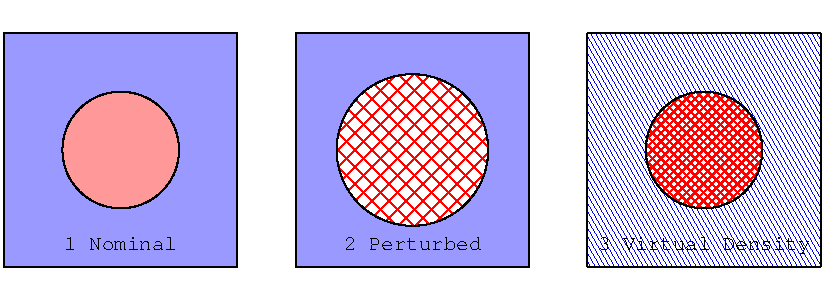
\includegraphics[height=2in]{./img/threeStates.pdf}
    \caption{For fuel radial expansion, the (left) nominal state expands to the (middle) perturbed state, which is physically similar to the (right) virtual density state.}
    \label{fig:threeStates}
\end{figure}
The original fuel and coolant densities are depicted in the nominal state.
Transitioning to the perturbed state, coolant is displaced by an expanding fuel and the fuel density is decreased in order to conserve fuel mass.
Transitioning to the virtual density state, fuel is contracted, coolant is expanded, and densities are changed inversely with the relative dimensional changes -- $\rho_i\ell_i$ is preserved for each component.
The result is a state which has the \textbf{same geometry} as the nominal state, but is \textbf{physically similar} to the perturbed state.

Virtual density theory allows a \textbf{geometric perturbation}, such as fuel rod radial expansion to be approximated with \textbf{density perturbations}.
If the geometric perturbation is space-dependent, density perturbations may be performed according to the same space-dependence.
For each geometric perturbation, there is a unique, physically similar, virtual density perturbation.
With this approach, only one perturbation can be assessed in a direct simulation; if 20 geometric perturbations are of interest, one nominal and 20 perturbed simulations must be performed \cite{reed2012vdp}.

\subsection{ Simulation of geometric perturbations with sensitivity theory and virtual density theory }

Sensitivity theory is a powerful and rigorous tool for quantifying the impact of nuclear data or material density perturbations upon the multiplication factor.
Recently, adjoint methods were added to MCNP \cite{mcnp6} adding sensitivity tools to a continuous-energy transport simulator.
These sensitivity tools allow sensitivity coefficients to be extracted for \textbf{all} materials present in the model simultaneously, with a single modified transport calculation.
With just a little bit of work, these material density sensitivities may be transformed into material density coefficients of reactivity.

If perturbations can be assumed linear -- linear coefficients of reactivity ($\alpha_p$) accurately describe the relation between reactivity ($\rho_k$) and the size of a perturbation ($p$) -- then reactivity deviations are proportional to the relative magnitude of the perturbation:
\begin{equation}
    \alpha_p
    \equiv \frac{\partial\rho_k}{\partial p}
    , \qquad
    \Delta\rho_{k,p}
    \approx \alpha_p \Delta p
    .
\end{equation}
Furthermore, using the definitions of reactivity and sensitivity, a coefficient of reactivity with respect to $p$ may be directly calculated from the sensitivity coefficient of $p$ ($S_p$):
\begin{equation}
    \label{eqn:essToRho}
    \alpha_p
    = \frac{k}{p} S_p
    , \qquad
    \Delta\rho_{k,p}
    \approx 
    \frac{\Delta p}{p} k S_p
    .
\end{equation}

In the current state of MCNP, sensitivity coefficients can be binned over neutron energy, isotope, and reaction type, but not space or neutron direction of travel.
However, with some small modifications of the nuclear data directory file, spatial binning may also be extracted, because MCNP treats `Material-dependent' sensitivities as material suffix sensitivities.
By segmenting materially uniform regions and pointing its sections to distinct nuclear data suffixes (which point to the exact same nuclear data) `material-dependent' material density sensitivities may be mapped to space-dependent material density sensitivities.

The final step is to recognize that, through virtual density theory, the effect that changes in material density have upon reactivity may be related those from changes in dimension.
With the combination of sensitivity theory, spatial segmentation and redundant nuclear data suffixes, and virtual density theory, any number of spatially dependent perturbations may be simulated with a single transport calculation and linear summation of sensitivities.

\section{ Methodology }

Here is the procedure for calculating any number of spatially dependent dimensional perturbations with a single transport calculation and linear summations which are tailored to each perturbation:
\begin{enumerate}
    \item Identify the components of each region which will undergo different dimensional perturbation
    \item Segment regions accordingly and assign them distinct nuclear data suffixes which point to the same underlying nuclear data
    \item Perform one transport calculation for the system at nominal conditions and estimate its space-dependent material density sensitivity coefficients
    \item Convert each of these material density sensitivity coefficients to material density coefficients of reactivity
    \item For each scenario with multiple dimensional perturbations
    \begin{enumerate}
        \item Determine the dimensional changes which will occur for each spatial region
        \item Use virtual density theory to calculate the virtual densities which return dimensions to their nominal states and preserve mean-free-paths (Equation \ref{eqn:virtualDensity})
        \item Take the summation over all spatial regions, of the material density changes with their corresponding material density coefficients of reactivity (Equation \ref{eqn:essToRho})
        \item The result is the combined reactivity deviation for the scenario
    \end{enumerate}
\end{enumerate}

\section{ Results }

FIXME

\section{ Conclusions }

FIXME

\bibliography{virtualDensity}

\end{document}
